\begin{figure}
  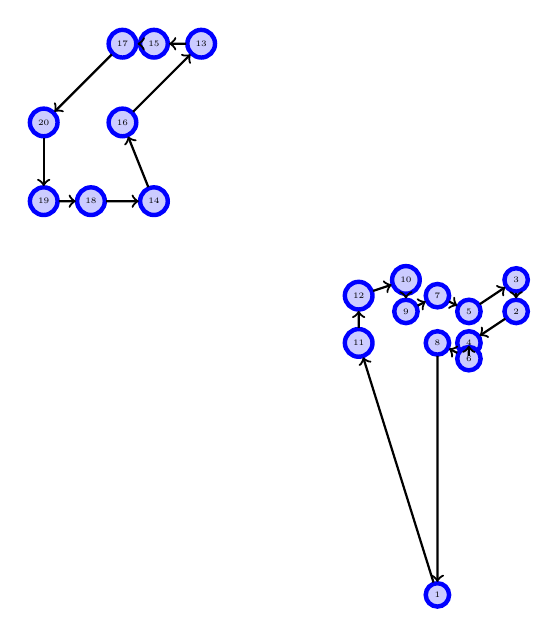
\begin{tikzpicture}[scale=0.2, ultra thick, node_style/.style={circle,draw=blue,fill=blue!20!,scale=0.6,font=\tiny},edge_style/.style={draw=black, thick,font=\tiny}]
      \draw
        (40.0, 50.0) node[node_style] (1){1}
        (45.0, 68.0) node[node_style] (2){2}
        (45.0, 70.0) node[node_style] (3){3}
        (42.0, 66.0) node[node_style] (4){4}
        (42.0, 68.0) node[node_style] (5){5}
        (42.0, 65.0) node[node_style] (6){6}
        (40.0, 69.0) node[node_style] (7){7}
        (40.0, 66.0) node[node_style] (8){8}
        (38.0, 68.0) node[node_style] (9){9}
        (38.0, 70.0) node[node_style] (10){10}
        (35.0, 66.0) node[node_style] (11){11}
        (35.0, 69.0) node[node_style] (12){12}
        (25.0, 85.0) node[node_style] (13){13}
        (22.0, 75.0) node[node_style] (14){14}
        (22.0, 85.0) node[node_style] (15){15}
        (20.0, 80.0) node[node_style] (16){16}
        (20.0, 85.0) node[node_style] (17){17}
        (18.0, 75.0) node[node_style] (18){18}
        (15.0, 75.0) node[node_style] (19){19}
        (15.0, 80.0) node[node_style] (20){20};
      \begin{scope}[->]
        \draw[edge_style] (1) to (11);
        \draw[edge_style] (2) to (4);
        \draw[edge_style] (3) to (2);
        \draw[edge_style] (4) to (6);
        \draw[edge_style] (5) to (3);
        \draw[edge_style] (6) to (8);
        \draw[edge_style] (7) to (5);
        \draw[edge_style] (8) to (1);
        \draw[edge_style] (9) to (7);
        \draw[edge_style] (10) to (9);
        \draw[edge_style] (11) to (12);
        \draw[edge_style] (12) to (10);
        \draw[edge_style] (13) to (15);
        \draw[edge_style] (14) to (16);
        \draw[edge_style] (15) to (17);
        \draw[edge_style] (16) to (13);
        \draw[edge_style] (17) to (20);
        \draw[edge_style] (18) to (14);
        \draw[edge_style] (19) to (18);
        \draw[edge_style] (20) to (19);
      \end{scope}
    \end{tikzpicture}
  \caption{test}\label{fig:soln}
\end{figure}